\appendix
\renewcommand{\thesection}{\Alph{section}}
\addcontentsline{toc}{section}{Appendix}
\OnehalfSpacing
%%%%%%%%%%%%%%%%%%%%%%%%%%%%%%%%%%%%%%%%

\section*{Appendix}
\bigskip
\textbf{The geometry of the celestial sphere}
\bigskip

\begin{figure}[!htbp]
    \centering
    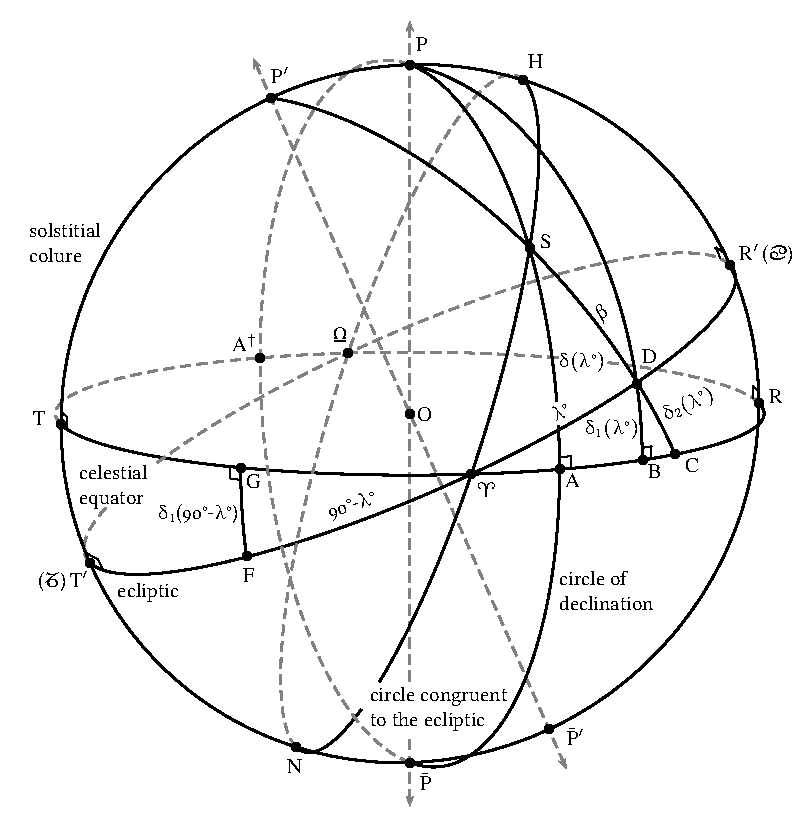
\includegraphics[width=\textwidth]{Images/Pstricks_drawing_declination_persian_sanskrit.pdf}
    \captionsetup{labelformat=empty}
    \caption{The celestial sphere showing the different spherical triangles inscribed by the celestial equator, the ecliptic, a great circle congruent to the ecliptic and passing through the celestial object, and their different secondary circles.}
    \label{celestial_sphere_drawing}
\end{figure}
\clearpage

\begin{sidewaystable}[htb]
% \caption{Technical (astronomical) terms in Persian and Sanskrit}
\label{sanskrit_persian_technical_terms_table_1}
\centering
\renewcommand*{\arraystretch}{1.75}
\renewcommand\tabularxcolumn[1]{m{#1}}%For vertical centring of object
\begin{tabularx}{\textwidth}{|c|>{\setlength{\baselineskip}{1.2\baselineskip}\raggedright\arraybackslash}X|}
\hline
\textbf{Object} & \textbf{Description}\\
\hline\hline
O& \textbf{centre of the celestial sphere}\\\hline
%
S&
\gls{celestial_object}$\enskip$  \tfarsi{کوکب} (\kawkab)$\enskip$ \tsans{nabhoga} (\textit{nabhoga}); \tsans{dyucara} (\textit{dyucara}); \tsans{bha} (\textit{bha}) \\\hline
%
P$\bar{\text{P}}$&
\gls{celestial_pole}$\enskip$ \tsans{vi.suvat-dhruva} (\textit{viṣuvat-dhruva}) \\\hline
%
P$'\bar{\text{P}}'$&
\gls{ecliptic_pole}$\enskip$ \tsans{kadamba} (\textit{kadamba}) \\\hline
%
\Aries\ \& \Libra &
\gls{pair_equinoctial_points}$\enskip$ \tsans{vi.suvat-dvaya} (\textit{viṣuvat-dvaya})\\\hline
%
R$'$ (\Cancer) \& T$'$ (\Capricorn) &
\textbf{pair of solstitial points}\\\hline
%%%%%%%%%%%%%
$\odot$ \Aries R \Libra T&
\gls{celestial_equator}$\enskip$  \tfarsi{معدّل النها}  (\muaddil\ \alnahar)$\enskip$ \tsans{vi.suva-v.rtta} (\textit{viṣuva-vṛtta}) \\\hline
%
$\odot$ \Aries R$'$ \Libra T$'$&
\gls{ecliptic}$\enskip$  \tfarsi{فلك البروج} (\falak\ \alburuj)$\enskip$ \tsans{bhavana-cakra} (\textit{bhavana-cakra}) \\\hline
%
$\odot$ \Aries SH \Libra N&
\gls{circle_congruent_ecliptic}$\enskip$ \tsans{bhacakra-sad.r"sa-v.rtta} (\textit{bhacakra-sadṛśa-vṛtta}); \tsans{bhacakra-sad.rk.sa-v.rtta} (\textit{bhacakra-sadṛkṣa-vṛtta}); \tsans{bhav.rtta-sad.r"sa-v.rtta} (\textit{bhavṛtta-sadṛśa-vṛtta}) \\\hline
%
$\odot$ P$\bar{\text{P}}'\bar{\text{P}}$P$'$&
\glslink{solstitial_colure}{circle belonging to the solstice}$\enskip$  \tsans{aayana-v.rtta} (\textit{āyana-vṛtta})$\quad$ 
\glslink{solstitial_colure}{circle passing through the four poles}$\enskip$ \tfarsi{دایرهٔ ماره باقطاب اربعه} (\textit{\dayiri\idafavowel\ \marri\ \biaqtab\idafaconsonant\ \arbai})$\enskip$ 
\tsans{dhruva-catu.ska-yaata-v.rtta} (\textit{dhruva-catuṣka-yāta-vṛtta})\\\hline
%
$\odot$ PSA$\bar{\text{P}}$A$^\dagger$& \gls{circle_of_declination} \tsans{kraanti-suutra} (\textit{krānti-sūtra})\\\hline
%
\rotatebox[origin=c]{90}{\Large \Rightcircle} PR\Aries T\Libra & \gls{celestial_hemisphere}$\enskip$ \tsans{gola} (\textit{gola}), towards the north \tsans{uttaraa-di"s} (\textit{uttarā-diś})\\\hline
%
\rotatebox[origin=c]{-90}{\Large \Rightcircle} $\bar{\text{P}}$T\Libra R\Aries & \gls{celestial_hemisphere}$\enskip$ \tsans{gola} (\textit{gola}), towards the south \tsans{yaamyaa-di"s} (\textit{yāmyā-diś})\\\hline
\end{tabularx}
\end{sidewaystable}

\newpage

\begin{sidewaystable}[htb]
% \caption{Technical (astronomical) terms in Persian and Sanskrit}
\label{sanskrit_persian_technical_terms_table_2}
\centering
\renewcommand*{\arraystretch}{1.75}
\renewcommand\tabularxcolumn[1]{m{#1}}%For vertical centring of object
\begin{tabularx}{\textwidth}{|c|>{\setlength{\baselineskip}{1.2\baselineskip}\raggedright\arraybackslash}X|}
\hline
\textbf{Object} & \textbf{Description}\\
\hline\hline
$\wideparen{\text{DS}}$&
\gls{latitude_celestial_object}$\enskip$ \tfarsi{عرض کوکب} (\ard\idafaconsonant\ \kawkab)
$\enskip$
\tsans{khagasya baa.na} (\textit{khagasya bāṇa})\\\hline
%
$\wideparen{\text{BD}}$& \gls{declination_degree_celestial_object}$\enskip$\tfarsi{میل درجه كوكب} (\mayl\idafaconsonant\ \daraji\idafavowel\ \kawkab)$\enskip$
\tsans{khagasya kraanti} (\textit{khagasya krānti}) \\\hline
%
$\wideparen{\text{RR}'}$& \gls{maximum_declination}, \ie \textbf{obliquity of the ecliptic}$\enskip$\tfarsi{میل کلّی} (\mayl\idafaconsonant\ \kulli)$\enskip$
\tsans{parama-kraanti} (\textit{parama-kraanti})\\\hline
%
$\wideparen{\text{CD}}$&
\gls{second_declination_degree}$\enskip$ \tfarsi{میل ثاني درجه} (\mayl\idafaconsonant\ \thani\idafavowel\ \daraji)
$\quad$
\gls{other_declination}$\enskip$ \tsans{anyatara-apama} (\textit{anyatara-apama}) \\\hline
%
$\wideparen{\text{AS}}$&
\gls{distance_celestial_object}$\enskip$ \tfarsi{بعد كواكب از معدّل النها} (\bud\idafaconsonant\ \kawkab\ \az\ \muaddil\ \alnahar)
\newline
\gls{true_declination}$\enskip$ \tsans{spa.s.ta-kraanti} (\textit{spaṣṭa-krānti})\\\hline
%
$\wideparen{\text{CS}}$&
\gls{argument_of_distance}$\enskip$ \tfarsi{حصّهٔ بعد} (\hissi\idafavowel\ \bud)
$\quad$
\gls{curve_true_declination}$\enskip$
\tsans{sphu.ta-apama-a"nka} (\textit{sphuṭa-apama-aṅka}) \\\hline
%
$\wideparen{\text{\Aries D}}$&
\gls{distance_degree_celestial_object_nearest_equinox}$\enskip$ \tfarsi{بعد درجه کوکب از اعتدال اقرب}  \newline(\textit{\bud\idafaconsonant\ \daraji\idafavowel\ \kawkab\ \az\ \itidal\idafaconsonant\ \aqrab}) 
$\quad$
\gls{degree_celestial_object}$\enskip$ \tfarsi{درجه کوکب} (\daraji\idafavowel\ \kawkab) \newline
\gls{arc_ecliptic_longitude_celestial_object}$\enskip$
\tsans{khagasya bhujaa} (\textit{khagasya bhujā}) \\\hline
%
$\wideparen{\text{DR}'}$&
\gls{distance_degree_celestial_object_nearest_solstice}$\enskip$
\tfarsi{بعد درجه کوکب از انقلاب اقرب} (\textit{\bud\idafaconsonant\ \daraji\idafavowel\ \kawkab\ \az\ \inqilab\idafaconsonant\ \aqrab})$\quad$
\gls{arc_complementary_ecliptic_longitude_celestial_object}$\enskip$ \tsans{khagasya ko.ti} (\textit{khagasya koṭi})\\\hline
%
$\wideparen{\text{\Aries S}}$&
\gls{congruent_bhuja}$\enskip$
\tsans{sad.r"s-bhujaa} (\textit{sadṛś-bhujā}); \tsans{sad.rk.sa-baahu} (\textit{sadṛkṣa-bāhu})\\\hline
%
$\wideparen{\text{SH}}$&
\gls{distance_celestial_object_solstice}$\enskip$
\tfarsi{بعد کوکب از
\tfarsib{دایرهٔ ماره باقطاب اربعه}} (\textit{\bud\idafaconsonant\ \kawkab\ \az\ \guillemotleft\dayiri\idafavowel\ \marri\ \biaqtab\idafaconsonant\ \arbai\guillemotright})$\quad$
\gls{congruent_koti}$\enskip$
\tsans{sad.r"s-ko.ti} (\textit{sadṛś-koṭi})\\\hline
%
$\wideparen{\text{R}'\text{H}}$&
\gls{first_arc}$\enskip$
\tfarsi{قوس اوّل} (\qaws\idafaconsonant\ \avval)$\quad$
\gls{maximum_latitude}$\enskip$
\tsans{para-i.su} (\textit{para-iṣu}); \tsans{para-"sara} (\textit{para-śara})\\\hline
%
$\wideparen{\text{R}\text{H}}$&
\gls{second_arc}$\enskip$
\tfarsi{قوس دوم} (\qaws\idafaconsonant\ \duvum)$\quad$
\gls{maximum_true_declination}$\enskip$
\tsans{para-sphu.ta-apama} (\textit{para-sphuṭa-apama})\\\hline
%
$\wideparen{\text{GF}}$&
\gls{inverse_declination}$\enskip$
\tfarsi{میل منکوس درجه كوكب} (\mayl\idafaconsonant\ \mankus\idafaconsonant\ \daraji\idafavowel\ \kawkab)\newline \textsc{note}: δ\textsubscript{1}(λ\degree + 90\degree) $\longleftrightarrow$ δ\textsubscript{1}(90\degree - λ\degree)\\\hline
\end{tabularx}
\end{sidewaystable}
